
\section*{CHƯƠNG 2. PHÂN TÍCH HỆ THỐNG}
\setcounter{section}{2}
\setcounter{subsection}{0} %LƯU Ý MỖI LẦN THÊM CHƯƠNG MỚI CẦN THÊM CÂU NÀY ĐỂ RESET THỨ TỰ CỦA SUBSECTON VỀ 1
\setcounter{table}{0} % LƯU Ý SAU MỖI LẦN GỌI BẢNG HAY HÌNH ẢNH PHẢI THÊM CÂU NÀY ĐỂ RESET THỨ TỰ
\setcounter{figure}{0} %% LƯU Ý SAU MỖI LẦN GỌI BẢNG HAY HÌNH ẢNH PHẢI THÊM CÂU NÀY ĐỂ RESET THỨ TỰ
\addcontentsline{toc}{section}{\numberline{}CHƯƠNG 2. PHÂN TÍCH HỆ THỐNG}
Chương này sẽ trình bày chi tiết về quá trình phân tích hệ thống, dựa trên các yêu cầu đã được nêu trong Phần mở đầu và Chương 1. Quá trình này bao gồm các bước sau:\begin{adjustwidth}{1.5em}{}
  \begin{itemize}
    \item Thiết kế các thẻ CRC (Class - Responsibility - Collaboration Card) cùng các lớp dựa trên thông tin từ các sơ đồ use case chức năng của hệ thống
    \item Xây dựng sơ đồ lớp dựa trên các lớp đã được định nghĩa với thuộc tính và phương thức
    \item Sau khi đã xác định về phương thức cũng như thuộc tính các lớp cùng chức năng, bước tiếp theo sẽ thiết kế các sơ đồ tuần tự minh họa sự tương tác giữa các lớp 
          khi thực hiện chức năng cụ thể
  \end{itemize}
  \end{adjustwidth}
% \newpage
\subsection{Thẻ CRC (Class - Responsibility - Collaboration Card)}

\subsubsection{Thẻ CRC lớp Người dùng}
\begin{xltabular}{\textwidth}{
   >{\centering\arraybackslash}X 
  }
  \caption{\bfseries \fontsize{12pt}{0pt}\selectfont Thẻ CRC lớp Người dùng}
  % \label{table_api_news}
  \\
  \begin{tabularx}{0.9\textwidth}{X}
    Mặt trước thẻ
  \end{tabularx}
  \begin{tabularx}{0.9\textwidth}{|X|X|}
    \hline
    \textbf{Tên lớp:} Người dùng (User) & \textbf{ID:} 1 \\
    \hline
    \textbf{Mô tả:} Đối tượng mô tả thông tin người dùng & \textbf{Use case liên quan:}  Đăng ký tài khoản, Quản lý tài khoản cá nhân, Quản lý phân công bác sĩ - bệnh nhân\\
    \hline
    \textbf{Trách nhiệm (Responsibility):} & \textbf{Các lớp cộng tác (Collaboration):} \\
    Thêm, sửa, xóa thông tin người dùng 

    Lấy danh sách người dùng

    Lấy thông tin người dùng qua ID, tài khoản, chức vụ
    & 
    Tài khoản
    \\
    \hline
  \end{tabularx}
  \\ 
  \begin{tabularx}{0.9\textwidth}{X}
    Mặt sau thẻ
  \end{tabularx} 
  \begin{tabularx}{0.9\textwidth}{|X|X|}
    \hline
    \textbf{Thuộc tính (Attributes):} & \\
    id(uuid) 
    
    username(String)

    birth(Timestamps)

    phone\_number(String)
    & 
    image(String) 
    
    role(Integer) 
    
    created\_at(Timestamps)

    updated\_at(Timestamps)
    \\ \hline
  \end{tabularx}
  \\     
  \begin{tabularx}{0.9\textwidth}{|X|}
    \hline
   \textbf{Mối quan hệ (Relationships)} \\
    Tổng quát hóa (Generalize):  

    Toàn thể - Bộ phận (Aggregation):
    
    Liên kết (Association): Tài khoản, Phân công bác sĩ - bệnh nhân 
    \\
    \hline
  \end{tabularx}
  \end{xltabular}

  \subsubsection{Thẻ CRC lớp Tài khoản}
  \begin{xltabular}{\textwidth}{
    >{\centering\arraybackslash}X 
   }
   \caption{\bfseries \fontsize{12pt}{0pt}\selectfont Thẻ CRC lớp Tài khoản}
   % \label{table_api_news}
   \\
   \begin{tabularx}{0.9\textwidth}{X}
     Mặt trước thẻ
   \end{tabularx}
   \begin{tabularx}{0.9\textwidth}{|X|X|}
     \hline
     \textbf{Tên lớp:} Tài khoản (Account) & \textbf{ID:} 2 \\
      \hline
      \textbf{Mô tả:} Đối tượng mô tả thông tin tài khoản & \textbf{Use case liên quan:} Đăng ký, Đăng nhập/Đăng xuất, Quên mật khẩu, Quản lý tài khoản người dùng \\
      \hline
      \textbf{Trách nhiệm (Responsibility):} & \textbf{Các lớp cộng tác (Collaboration):} \\
      Đăng nhập/Đăng xuất hệ thống

      Đăng ký tài khoản

      Quên mật khẩu

      Chỉnh sửa thông tin tài khoản

      Lấy thông tin tài khoản qua email
      & 
      Token đăng nhập
      \\
     \hline
   \end{tabularx}
   \\ 
   \begin{tabularx}{0.9\textwidth}{X}
     Mặt sau thẻ
   \end{tabularx}
   \begin{tabularx}{0.9\textwidth}{|X|}
    \hline
    \textbf{Thuộc tính (Attributes):} \\
    id(String) 
    
    email(String)

    password(String)
    \\
    \hline
  \end{tabularx}
   \\     
   \begin{tabularx}{0.9\textwidth}{|X|}
     \textbf{Mối quan hệ (Relationships)} \\
     Tổng quát hóa (Generalize):  

     Toàn thể - Bộ phận (Aggregation):   
     
     Liên kết (Association): Người dùng, Token đăng nhập      \\
     \hline
   \end{tabularx}
   \end{xltabular}
   

\subsubsection{Thẻ CRC lớp Tài khoản phê duyệt}
  \begin{xltabular}{\textwidth}{
    >{\centering\arraybackslash}X 
  }
  \newpage
  \caption{\bfseries \fontsize{12pt}{0pt}\selectfont Thẻ CRC lớp Tài khoản phê duyệt}
  % \label{table_api_news}
  \\
  \begin{tabularx}{0.9\textwidth}{X}
    Mặt trước thẻ
  \end{tabularx}
  \begin{tabularx}{0.9\textwidth}{|X|X|}
    \hline
    \textbf{Tên lớp:} Tài khoản phê duyệt (Register) & \textbf{ID:} 3 \\
    \hline
    \textbf{Mô tả:} Đối tượng mô tả thông tin tài khoản đang chờ phê duyệt & \textbf{Use case liên quan:} Đăng ký, Quản lý tài khoản người dùng \\
    \hline
    \textbf{Trách nhiệm (Responsibility):} & \textbf{Các lớp cộng tác (Collaboration):} \\
    Lấy danh sách tài khoản đang chờ phê duyệt
    
    Đăng ký tài khoản

    Phê duyệt tài khoản
    & 
    Người dùng, Tài khoản
    \\
    \hline
  \end{tabularx}
  \\ 
  \begin{tabularx}{0.9\textwidth}{X}
    Mặt sau thẻ
  \end{tabularx}
  \begin{tabularx}{0.9\textwidth}{|X|X|}
    \hline
    \textbf{Thuộc tính (Attributes):} & \\
    id(String) 
    
    email(String)

    password(String)

    birth(Timestamps)

    gender(Integer)

    phone\_number(String)
    &
    image(String)

    status(Integer)

    infomation(String)

    role(Integer)

    created\_at(Timestamps)

    updated\_at(Timestamps)
    \\
    \hline
  \end{tabularx}
  \\     
  \begin{tabularx}{0.9\textwidth}{|X|}
    \textbf{Mối quan hệ (Relationships)} \\
    Tổng quát hóa (Generalize):  

    Toàn thể - Bộ phận (Aggregation):   
      
    Liên kết (Association): Người dùng, Tài khoản
    \\
    \hline
  \end{tabularx}
  \end{xltabular}

\subsubsection{Thẻ CRC lớp Token đăng nhập}
  \begin{xltabular}{\textwidth}{
    >{\centering\arraybackslash}X 
  }
  \caption{\bfseries \fontsize{12pt}{0pt}\selectfont Thẻ CRC lớp Token đăng nhập}
  % \label{table_api_news}
  \\
  \begin{tabularx}{0.9\textwidth}{X}
    Mặt trước thẻ
  \end{tabularx}
  \begin{tabularx}{0.9\textwidth}{|X|X|}
    \hline
    \textbf{Tên lớp:} Token đăng nhập (Token) & \textbf{ID:} 4  \\
    \hline
    \textbf{Mô tả:} Đối tượng mô tả thông tin token tài khoản & \textbf{Use case liên quan:} Đăng nhập/Đăng xuất \\
    \hline
    \textbf{Trách nhiệm (Responsibility):} & \textbf{Các lớp cộng tác (Collaboration):} \\
    Mô tả thông tin token tài khoản

    Tạo/xóa access token và refresh token khi đăng nhập/đăng xuất

    Xác thực token khi đăng nhập
    & 
    Tài khoản
    \\
    \hline
  \end{tabularx}
  \\
  \begin{tabularx}{0.9\textwidth}{X}
    Mặt sau thẻ
  \end{tabularx} 
  \begin{tabularx}{0.9\textwidth}{|X|X|}
    \hline
    \textbf{Thuộc tính (Attributes):} & \\
    id(String) 
    
    access\_token(String)
    
    refresh\_token(String) 
    & 
    
    created\_at(Timestamps)

    updated\_at(Timestamps)
    \\
    \hline
  \end{tabularx}
  \\     
  \begin{tabularx}{0.9\textwidth}{|X|}
    \textbf{Mối quan hệ (Relationships)} \\
    Tổng quát hóa (Generalize):

    Toàn thể - Bộ phận (Aggregation):
      
    Liên kết (Association): Tài khoản
    \\
    \hline
  \end{tabularx}
  \end{xltabular}

  \subsubsection{Thẻ CRC lớp Thiết bị}
  \begin{xltabular}{\textwidth}{
    >{\centering\arraybackslash}X 
  }
  \caption{\bfseries \fontsize{12pt}{0pt}\selectfont Thẻ CRC lớp Thiết bị}
  % \label{table_api_news}
  \\
  \begin{tabularx}{0.9\textwidth}{X}
    Mặt trước thẻ
  \end{tabularx}
  \begin{tabularx}{0.9\textwidth}{|X|X|}
    \hline
    \textbf{Tên lớp:} Thiết bị (Device) & \textbf{ID:} 5 \\
    \hline
    \textbf{Mô tả:} Đối tượng mô tả thông tin thiết bị & \textbf{Use case liên quan:} Quản lý thiết bị, Quản lý lịch sử đo bệnh nhân \\
    \hline
    \textbf{Trách nhiệm (Responsibility):} & \textbf{Các lớp cộng tác (Collaboration):} \\
    Mô tả thông tin thiết bị

    Lấy danh sách tất cả thiết bị

    Lấy danh sách thiết bị theo người dùng, bác sĩ
    
    Thêm, sửa, xóa thiết bị
    & 
    Người dùng, Thông số thiết bị 
    \\
    \hline
  \end{tabularx}
  \\ 
  \begin{tabularx}{0.9\textwidth}{X}
    Mặt sau thẻ
  \end{tabularx} 
  \begin{tabularx}{0.9\textwidth}{|X|X|}
    \hline
    \textbf{Thuộc tính (Attributes):} & \\
    id(String) 

    device\_name(String)

    infomation(String)

    device\_type(Integer)
    & 
    start\_date(Timestamps) 
    
    end\_date(Timestamps) 
    
    created\_at(Timestamps)

    updated\_at(Timestamps)
    \\
    \hline
  \end{tabularx}
  \\     
  \begin{tabularx}{0.9\textwidth}{|X|}
    \textbf{Mối quan hệ (Relationships)} \\
    Tổng quát hóa (Generalize):  

    Toàn thể - Bộ phận (Aggregation): Người dùng
      
    Liên kết (Association): Thông số thiết bị
    \\
    \hline
  \end{tabularx}
  \end{xltabular}
  \newpage
  \subsubsection{Thẻ CRC lớp Thông số thiết bị}
  \begin{xltabular}{\textwidth}{
    >{\centering\arraybackslash}X 
  }
  \caption{\bfseries \fontsize{12pt}{0pt}\selectfont Thẻ CRC lớp Thông số thiết bị}
  % \label{table_api_news}
  \\
  \begin{tabularx}{0.9\textwidth}{X}
    Mặt trước thẻ
  \end{tabularx}
  \begin{tabularx}{0.9\textwidth}{|X|X|}
    \hline
    \textbf{Tên lớp:} Thông số thiết bị (Device Detail) & \textbf{ID:} 6 \\
    \hline
    \textbf{Mô tả:} Đối tượng mô tả thông tin thông số thiết bị & \textbf{Use case liên quan:} Quản lý thiết bị\\
    \hline
    \textbf{Trách nhiệm (Responsibility):} & \textbf{Các lớp cộng tác (Collaboration):} \\
    Mô tả thông tin thông số thiết bị

    Lấy thông số theo thiết bị
    & 
    Thiết bị 
    \\
    \hline
  \end{tabularx}
  \\ 
  \begin{tabularx}{0.9\textwidth}{X}
    Mặt sau thẻ
  \end{tabularx} 
  \begin{tabularx}{0.9\textwidth}{|X|X|}
    \hline
    \textbf{Thuộc tính (Attributes):} & \\
    id(String) 
  
    detail\_name(String)

    infomation(String)
    
    value(Integer)
    & 
    detail\_type(Integer)
    
    created\_at(Timestamps)

    updated\_at(Timestamps)
    \\
    \hline
  \end{tabularx}
  \\     
  \begin{tabularx}{0.9\textwidth}{|X|}
    \textbf{Mối quan hệ (Relationships):} \\
    Tổng quát hóa (Generalize):  

    Toàn thể - Bộ phận (Aggregation): 
    
    Liên kết (Association): Thiết bị
    \\
    \hline
  \end{tabularx}
  \end{xltabular}

\subsubsection{Thẻ CRC lớp Bản ghi}
  \begin{xltabular}{\textwidth}{
    >{\centering\arraybackslash}X 
  }
  \caption{\bfseries \fontsize{12pt}{0pt}\selectfont Thẻ CRC lớp Bản ghi}
  % \label{table_api_news}
  \\
  \begin{tabularx}{0.9\textwidth}{X}
    Mặt trước thẻ
  \end{tabularx}
  \begin{tabularx}{0.9\textwidth}{|X|X|}
    \hline
    \textbf{Tên lớp:} Bản ghi (Record) & \textbf{ID:} 7 \\
    \hline
    \textbf{Mô tả:} Đối tượng mô tả thông tin bản ghi & \textbf{Use case liên quan:} Quản lý lịch sử đo bệnh nhân \\
    \hline
    \textbf{Trách nhiệm (Responsibility):} & \textbf{Các lớp cộng tác (Collaboration):} \\
    Mô tả thông tin bản ghi 

    Lấy danh sách tất cả bản ghi

    Lấy danh sách bản ghi theo người dùng, thiết bị

    Thêm, sửa, xóa thông tin bản ghi

    Đọc, tải bản ghi
    & 
    Người dùng, Thiết bị
    \\
    \hline
  \end{tabularx}
  \\ 
  \begin{tabularx}{0.9\textwidth}{X}
    Mặt sau thẻ
  \end{tabularx}
  \begin{tabularx}{0.9\textwidth}{|X|X|}
    \hline
    \textbf{Thuộc tính (Attributes):} & \\
    id(String) 

    start\_time(Timestamps)

    end\_time(Timestamps) 
    & 
    
    data\_rec\_url(String) 
    
    created\_at(Timestamps)

    updated\_at(Timestamps)
    \\
    \hline
  \end{tabularx}
  \\     
  \begin{tabularx}{0.9\textwidth}{|X|}
    \textbf{Mối quan hệ (Relationships):} \\
    Tổng quát hóa (Generalize):  

    Toàn thể - Bộ phận (Aggregation): 
    
    Liên kết (Association):  Người dùng, Thiết bị
    \\
    \hline
  \end{tabularx}
  \end{xltabular}

\subsubsection{Thẻ CRC lớp Phân công bác sĩ - bệnh nhân}
  \begin{xltabular}{\textwidth}{
    >{\centering\arraybackslash}X 
  }
  \caption{\bfseries \fontsize{12pt}{0pt}\selectfont Thẻ CRC lớp Phân công bác sĩ - bệnh nhân}
  % \label{table_api_news}
  \\
  \begin{tabularx}{0.9\textwidth}{X}
    Mặt trước thẻ
  \end{tabularx}
  \begin{tabularx}{0.9\textwidth}{|X|X|}
    \hline
    \textbf{Tên lớp:} Phân công bác sĩ - bệnh nhân (Patient Doctor Assignment) & \textbf{ID:} 8 \\
    \hline
    \textbf{Mô tả:} Đối tượng mô tả thông tin quản lý giữa bác sĩ và bệnh nhân & \textbf{Use case liên quan:} Quản lý phân công bác sĩ - bệnh nhân \\
    \hline
    \textbf{Trách nhiệm (Responsibility):} & \textbf{Các lớp cộng tác (Collaboration):} \\
    Mô tả thông tin quan lý giữa bác sĩ và bệnh nhân

    Lấy danh sách tất cả phân công

    Lấy danh sách phân công theo bác sĩ, bệnh nhân

    Phân công bệnh nhân theo bác sĩ
    & 
    Người dùng
    \\
    \hline
  \end{tabularx}
  \\ 
  \begin{tabularx}{0.9\textwidth}{X}
    Mặt sau thẻ
  \end{tabularx} 
  \begin{tabularx}{0.9\textwidth}{|X|}
    \hline
    \textbf{Thuộc tính (Attributes):} \\
    id(String) 

    start\_date(Timestamps) 
          
    created\_at(Timestamps)

    updated\_at(Timestamps)
    \\
    \hline
  \end{tabularx}
  \\     
  \begin{tabularx}{0.9\textwidth}{|X|}
    \textbf{Mối quan hệ (Relationships):} \\
    Tổng quát hóa (Generalize):

    Toàn thể - Bộ phận (Aggregation): 
    
    Liên kết (Association): Người dùng
    \\
    \hline
  \end{tabularx}
  \end{xltabular}

\newpage

  \subsubsection{Thẻ CRC lớp Thành viên tham gia hội thoại}
  \begin{xltabular}{\textwidth}{
    >{\centering\arraybackslash}X 
  }
  \caption{\bfseries \fontsize{12pt}{0pt}\selectfont Thẻ CRC lớp Tài khoản}
  % \label{table_api_news}
  \\
  \begin{tabularx}{0.9\textwidth}{X}
    Mặt trước thẻ
  \end{tabularx}
  \begin{tabularx}{0.9\textwidth}{|X|X|}
    \hline
    \textbf{Tên lớp:} Thành viên tham gia hội thoại & \textbf{ID:} 11 \\
    \hline
    \textbf{Mô tả:} Đối tượng mô tả thông tin Thành viên tham gia hội thoại & \textbf{Use case liên quan:} Quản lý dịch vụ nhắn tin; Hỏi, tư vấn từ trợ lý ảo \\
    \hline
    \textbf{Trách nhiệm (Responsibility):} & \textbf{Các lớp cộng tác (Collaboration):} \\
    Thông tin Thành viên tham gia hội thoại

    Lấy danh sách thành viên theo hội thoại
    & 
    Cuộc hội thoại 
    \\
    \hline
  \end{tabularx}
  \\ 
  \begin{tabularx}{0.9\textwidth}{X}
    Mặt sau thẻ
  \end{tabularx} 
  \begin{tabularx}{0.9\textwidth}{|X|}
    \hline
    \textbf{Thuộc tính (Attributes):} \\
    id(String) 

    status\_notify(Integer)

    role(Integer)

    seen(Boolean)
    \\
    \hline
  \end{tabularx}
  \\     
  \begin{tabularx}{0.9\textwidth}{|X|}
    \textbf{Mối quan hệ (Relationships):} \\
    Tổng quát hóa (Generalize):  

    Toàn thể - Bộ phận (Aggregation): 
    
    Liên kết (Association): Người dùng, Cuộc hội thoại
    \\
    \hline
  \end{tabularx}
  \end{xltabular}

  \subsubsection{Thẻ CRC lớp Cuộc hội thoại}
  \begin{xltabular}{\textwidth}{
    >{\centering\arraybackslash}X 
  }
  \caption{\bfseries \fontsize{12pt}{0pt}\selectfont Thẻ CRC lớp Cuộc hội thoại}
  % \label{table_api_news}
  \\
  \begin{tabularx}{0.9\textwidth}{X}
    Mặt trước thẻ
  \end{tabularx}
  \begin{tabularx}{0.9\textwidth}{|X|X|}
    \hline
    \textbf{Tên lớp:} Cuộc hội thoại & \textbf{ID:} 12 \\
    \hline
    \textbf{Mô tả:} Đối tượng mô tả thông tin Thành viên tham gia hội thoại & \textbf{Use case liên quan:} Quản lý dịch vụ nhắn tin; Hỏi, tư vấn từ trợ lý ảo \\
    \hline
    \textbf{Trách nhiệm (Responsibility):} & \textbf{Các lớp cộng tác (Collaboration):} \\
    Mô tả thông tin cuộc hội thoại

    Thêm, xóa hội thoại
    & 

    \\
    \hline
  \end{tabularx}
  \\ 
  \begin{tabularx}{0.9\textwidth}{X}
    Mặt sau thẻ
  \end{tabularx} 
  \begin{tabularx}{0.9\textwidth}{|X|}
    \hline
    \textbf{Thuộc tính (Attributes):} \\
    conversation\_id(String) 
    
    name(String)

    type(Integer)

    avatar\_url(String)
    \\
    \hline
  \end{tabularx}
  \\     
  \begin{tabularx}{0.9\textwidth}{|X|}
    \textbf{Mối quan hệ (Relationships):} \\
    Tổng quát hóa (Generalize):  

    Toàn thể - Bộ phận (Aggregation): 
    
    Liên kết (Association): Thành viên tham gia hội thoại, Tin nhắn 
    \\
    \hline
  \end{tabularx}
  \end{xltabular}

\subsubsection{Thẻ CRC lớp Tin nhắn}
  \begin{xltabular}{\textwidth}{
    >{\centering\arraybackslash}X 
  }
  \caption{\bfseries \fontsize{12pt}{0pt}\selectfont Thẻ CRC lớp Tin nhắn}
  % \label{table_api_news}
  \\
  \begin{tabularx}{0.9\textwidth}{X}
    Mặt trước thẻ
  \end{tabularx}
  \begin{tabularx}{0.9\textwidth}{|X|X|}
    \hline
    \textbf{Tên lớp:} Tin nhắn & \textbf{ID:} 13 \\
    \hline
    \textbf{Mô tả:} Đối tượng mô tả thông tin Tin nhắn & \textbf{Use case liên quan:} Quản lý dịch vụ nhắn tin; Hỏi, tư vấn từ trợ lý ảo \\
    \hline
    \textbf{Trách nhiệm (Responsibility):} & \textbf{Các lớp cộng tác (Collaboration):} \\
    Mô tả thông tin Tin nhắn

    Xem/gửi tin nhắn

    Lấy danh sách tin nhắn theo hội thoại, người gửi
    & 
    Thành viên tham gia hội thoại, Cuộc hội thoại, Tệp đính kèm
    \\
    \hline
  \end{tabularx}
  \\ 
  \begin{tabularx}{0.9\textwidth}{X}
    Mặt sau thẻ
  \end{tabularx} 
  \begin{tabularx}{0.9\textwidth}{|X|X|}
    \hline
    \textbf{Thuộc tính (Attributes):} & \\
    message\_id(String) 

    attachments(List)
    
    system\_message(Boolean)
    &
    pin(Boolean)

    pin\_time(Timestamps)

    reactions(List)
    \\
    \hline
  \end{tabularx}
  \\     
  \begin{tabularx}{0.9\textwidth}{|X|}
    \textbf{Mối quan hệ (Relationships):} \\
    Tổng quát hóa (Generalize):  

    Toàn thể - Bộ phận (Aggregation): 
    
    Liên kết (Association): Thành viên tham gia hội thoại, Cuộc hội thoại, Tệp đính kèm 
    \\
    \hline
  \end{tabularx}
  \end{xltabular}

  \subsubsection{Thẻ CRC lớp Tệp đính kèm}
  \begin{xltabular}{\textwidth}{
    >{\centering\arraybackslash}X 
  }
  \caption{\bfseries \fontsize{12pt}{0pt}\selectfont Thẻ CRC lớp Tệp đính kèm}
  % \label{table_api_news}
  \\
  \begin{tabularx}{0.9\textwidth}{X}
    Mặt trước thẻ
  \end{tabularx}
  \begin{tabularx}{0.9\textwidth}{|X|X|}
    \hline
    \textbf{Tên lớp:} Tệp đính kèm & \textbf{ID:} 14 \\
    \hline
    \textbf{Mô tả:} Đối tượng mô tả thông tin Tệp đính kèm tin nhắn & \textbf{Use case liên quan:} Quản lý dịch vụ nhắn tin \\
    \hline
    \textbf{Trách nhiệm (Responsibility):} & \textbf{Các lớp cộng tác (Collaboration):} \\
    Mô tả thông tin Tệp đính kèm

    Lấy thông tin tệp đính kèm theo tin nhắn, cuộc hội thoại
    & 
    Tin nhắn, Cuộc hội thoại
    \\
    \hline
  \end{tabularx}
  \\ 
  \begin{tabularx}{0.9\textwidth}{X}
    Mặt sau thẻ
  \end{tabularx} 
  \begin{tabularx}{0.9\textwidth}{|X|X|}
    \hline
    \textbf{Thuộc tính (Attributes):} & \\
    id(String) 

    content\_url(String)
    
    file\_name(String)
    &
    size(Integer)

    thumbnail\_url(String)

    type(Integer)
    \\
    \hline
  \end{tabularx}
  \\     
  \begin{tabularx}{0.9\textwidth}{|X|}
    \textbf{Mối quan hệ (Relationships):} \\
    Tổng quát hóa (Generalize):  

    Toàn thể - Bộ phận (Aggregation): 
    
    Liên kết (Association): Tin nhắn, Cuộc hội thoại 
    \\
    \hline
  \end{tabularx}
  \end{xltabular}


% \newpage
\subsection{Sơ đồ lớp}
  Dựa trên các thẻ CRC đã được mô tả ở phần trên, chúng em xin phép trình bày về sơ đồ lớp của hệ thống.
  \begin{figure}[H]
    \centering
    \includegraphics*[width = 16cm, height = 19cm]{Images/UML/UML.drawio.png}
    \caption[Sơ đồ lớp của hệ thống]{\bfseries \fontsize{12pt}{0pt}
    \selectfont Sơ đồ lớp của hệ thống}
    \label{UML}
  \end{figure}

  % Hình \ref*{UML} thể hiện các lớp trong hệ thống:
  % \begin{itemize}
  %   \item Lớp Account (Tài khoản): Lớp thể hiện cho cấu trúc của một account khi đăng ký sử dụng hệ thống, cung cấp các hàm và các biến để thực hiện chức năng đăng ký người dùng
  %   \item Lớp Register (Tài khoản phê duyệt): Lớp thể hiện cho cấu trúc của người dùng khi mới đăng ký, cung cấp các hàm, phương thức thao tác dữ liệu người dùng khi mới đăng ký
  %   \item Lớp User (Người dùng): Lớp thể hiện cho cấu trúc của người dùng sau khi đã đăng ký, cung cấp các hàm, phương thức liên quan đến dữ liệu người dùng sau đăng ký
  %   \item Lớp Token: Lớp thể hiện cho cấu trúc của một token, cung cấp biến, hàm để thao tác với người dùng khi thực hiện đăng ký, đăng nhập
  %   \item Lớp PatientDoctorAssignment (Phân công bác sĩ - bệnh nhân): Lớp thể hiện cho cấu trúc của một bảng phân công giữa bệnh nhân và bác sĩ, cung cấp các hàm, phương thức để lấy dữ liệu phân công bệnh nhân/bác sĩ
  %   \item Lớp Record (Bản ghi): Lớp thể hiện cho cấu trúc của một bản ghi record, cung cấp các hàm, phương thức để thực hiện liên quan đến các bản ghi dữ liệu sức khỏe của bệnh nhân
  %   \item Lớp Device (Thiết bị): Lớp thể hiện cho cấu trúc của một thiết bị, cung cấp các biến, hàm, phương thức để thực hiện liên quan đến thông tin các thiết bị sử dụng trong các ghi record
  %   \item Lớp DeviceDetail (Thông số thiết bị): Lớp thể hiện cho cấu trúc của chi tiết liên quan đến lớp thiết bị, cung cấp các hàm, phương thức để thực hiện thao tác với dữ liệu các thiết bị và các bản ghi record
  %   \item Lớp News (Tin tức): Lớp thể hiện cho cấu trúc của một tin tức, cung cấp các hàm, phương thức để lấy dữ liệu tin tức
  %   \item Lớp NewsCategories (Danh mục tin tức): Lớp thể hiện cho cấu trúc của một danh mục tin tức, cung cấp các hàm, phương thức để lấy dữ liệu từ danh mục tin tức
  %   \item Lớp Conversation (Cuộc hội thoại): Lớp thể hiện cho cấu trúc của một cuộc hội thoại, cung cấp các biến, hàm, phương thức để lấy dữ liệu liên quan đến cuộc hội thoại
  %   \item Lớp ConversationMember (Thành viên tham gia hội thoại): Lớp thể hiện cho cấu trúc của danh sách những người tham gia một cuộc hội thoại, cung cấp các hàm, phương thức để xử lý dữ liệu liên quan đến người dùng
  %   \item Lớp ConversationAttachment (Tệp đính kèm): Lớp thể hiện cho cấu trúc của danh sách những tệp được đính kém trong danh sách hội thoại, cung cấp các hàm, phương thức để xử lý các chức năng liên quan đến hội thoại
  %   \item Lớp Message (Tin nhắn): Lớp thể hiện cho cấu trúc của một message được sử dụng trong hội thoại, cung cấp các hàm, phương thức để xử lý dữ liệu trong cuộc hội thoại
  % \end{itemize}
% \newpage
\subsection{Sơ đồ tuần tự}
Để phân tích cụ thể hơn về từng luồng trong hệ thống thông qua sơ đồ use case và sơ đồ hoạt động, dưới đây là phần thiết kế
 về các sơ đồ tuần tự.

\subsubsection{Sơ đồ tuần tự đăng ký tài khoản}
\begin{figure}[H]
  \centering
  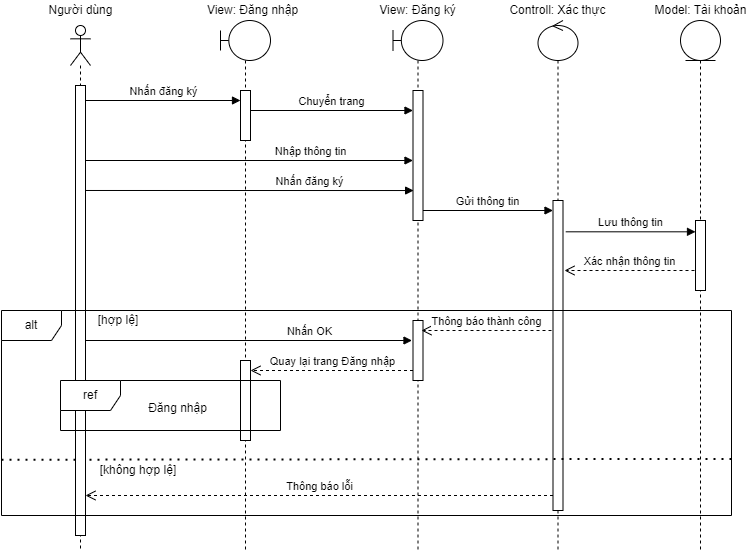
\includegraphics[width=10cm,height=12.5cm]{Images/sequence/sequence_register.png}
  \caption[Sơ đồ tuần tự đăng ký tài khoản]{\bfseries \fontsize{12pt}{0pt}
  \selectfont Sơ đồ tuần tự đăng ký tài khoản}
  \label{sequence_register} %đặt tên cho ảnh
\end{figure}
Sơ đồ tuần tự mô tả chi tiết quá trình người dùng đăng ký một tài khoản mới trên hệ thống. Người dùng sẽ phải gửi yêu cầu đăng ký, hệ thống sẽ được xử lý
bởi lớp Register, nếu có lỗi phát sinh hệ thống sẽ thông báo lõi cho người dùng. Nếu việc đăng ký thành công, lớp Register sẽ gửi thông báo 
chuyển sang phê duyệt tài khoản và trả về kết quả.  

\subsubsection{Sơ đồ tuần tự đăng nhập/xuất}
\begin{figure}[H]
  \centering
  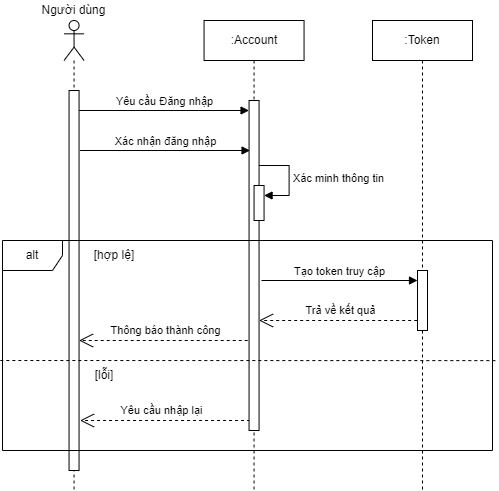
\includegraphics[width=12cm,height=11cm]{Images/sequence/sequence_login.png}
  \caption[Sơ đồ tuần tự đăng nhập]{\bfseries \fontsize{12pt}{0pt}
  \selectfont Sơ đồ tuần tự đăng nhập}
  \label{sequence_login} %đặt tên cho ảnh
\end{figure}
Sơ đồ tuần tự mô tả chi tiết quá trình đăng nhập trên hệ thống của người dùng. Người dùng sẽ phải gửi yêu cầu đăng nhập, hệ thống sẽ được xử lý
bởi lớp Account, nếu có lỗi sẽ trả về người dùng. Nếu việc đăng ký thành công, lớp Account sẽ gửi thông báo 
tạo token truy cập mới và thông báo thành công. 
\begin{figure}[H]
  \centering
  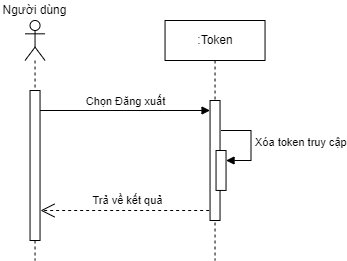
\includegraphics[width=9.5cm,height=6.5cm]{Images/sequence/sequence_logout.png}
  \caption[Sơ đồ tuần tự chức năng đăng xuất]{\bfseries \fontsize{12pt}{0pt}
  \selectfont Sơ đồ tuần tự chức năng đăng xuất}
  \label{sequence_logout} %đặt tên cho ảnh
\end{figure}
Sơ đồ tuần tự trên mô tả quá trình đăng xuất khỏi hệ thống. Người dùng sẽ gửi yêu cầu đăng xuất, yêu cầu sẽ được xử lý
bởi lớp Token. Lớp Token sẽ xóa thông tin token truy cập và trả về kết quả đăng xuất.

\subsubsection{Sơ đồ tuần tự quên mật khẩu}
\begin{figure}[H]
  \centering
  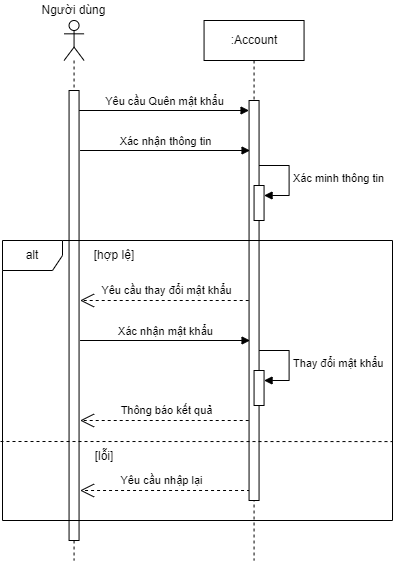
\includegraphics[width=10cm,height=13.5cm]{Images/sequence/sequence_forgot_password.png}
  \caption[Sơ đồ tuần tự quên mật khẩu]{\bfseries \fontsize{12pt}{0pt}
  \selectfont Sơ đồ tuần tự quên mật khẩu}
  \label{sequence_forgot_pass} %đặt tên cho ảnh
\end{figure}
Sơ đồ tuần tự trên mô tả chi tiết quá trình lấy mật khẩu mới trên hệ thống. Người dùng sẽ gửi email đã đăng ký tài khoản, gửi yêu cầu
lấy lại mật khẩu. Yêu cầu sẽ được xử lý bởi lớp Account, nếu có lỗi phát sinh sẽ hiển thị lên màn hình và yêu cầu người dùng nhập lại. Lớp Account sẽ gửi một mã xác thực
đến email, người dùng sẽ nhập mã xác thực và thay đổi mật khẩu mới. Nếu việc thay đổi thành công, lớp Account sẽ gửi thông báo thành công và chuyển sang đăng nhập.

\subsubsection{Sơ đồ tuần tự quản lý tài khoản cá nhân}
\begin{figure}[H]
  \centering
  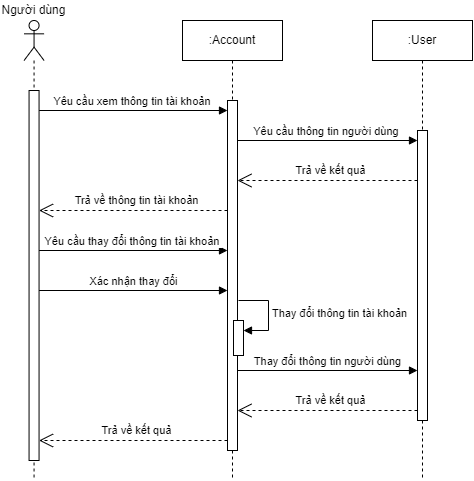
\includegraphics[width=12cm,height=12cm]{Images/sequence/sequence_manage_info.png}
  \caption[Sơ đồ tuần tự chức năng quản lý tài khoản cá nhân]{\bfseries \fontsize{12pt}{0pt}
  \selectfont Sơ đồ tuần tự chức năng quản lý tài khoản cá nhân}
  \label{sequence_account} %đặt tên cho ảnh
\end{figure}
Sơ đồ tuần tự trên mô tả chi tiết quá trình người dùng lấy và thay đổi thông tin tài khoản trên hệ thống. Người dùng thay đổi thông tin cá nhân và gửi yêu cầu tới hệ thống, 
yêu cầu sẽ được xử lý bởi 2 lớp Account và lớp User, nếu có lỗi phát sinh sẽ thông báo lỗi cho người dùng. Nếu việc thay đổi thành công, lớp Account sẽ gửi thông báo 
thành công.  

\subsubsection{Sơ đồ tuần tự chức năng quản lý dữ liệu đo}
\begin{figure}[H]
  \centering
  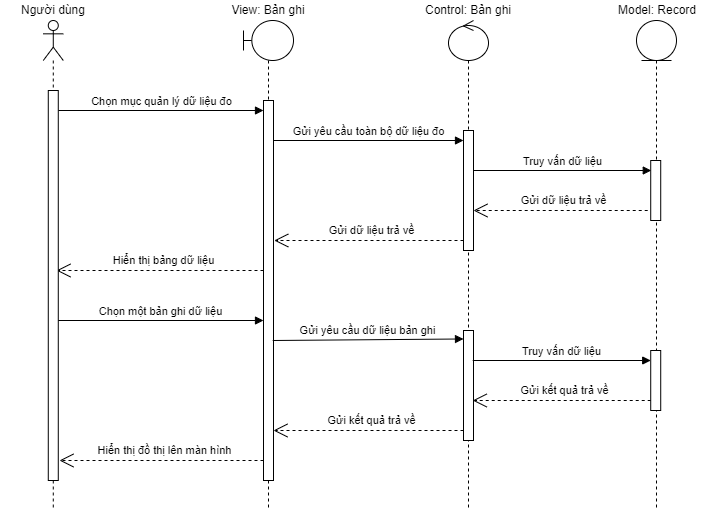
\includegraphics[width=10cm,height=6.5cm]{Images/sequence/sequence_manage_record.png}
  \caption[Sơ đồ tuần tự chức năng xem danh sách phiên đo]{\bfseries \fontsize{12pt}{0pt}
  \selectfont Sơ đồ tuần tự chức năng xem danh sách phiên đo}
  \label{sequence_manage_record} %đặt tên cho ảnh
\end{figure}
Sơ đồ tuần tự trên mô tả chi tiết quá trình người dùng lấy danh sách lịch sử đo trên hệ thống. Người dùng gửi yêu cầu xem danh sách phiên đo, 
yêu cầu sẽ được xử lý bởi lớp Record, hiện danh sách các bản ghi phiên đo cho người dùng.

\begin{figure}[H]
  \centering
  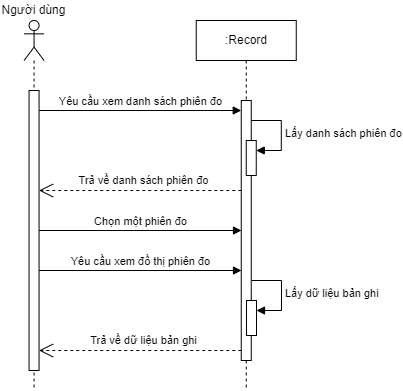
\includegraphics[width=10.5cm,height=10cm]{Images/sequence/sequence_manage_chart_record.png}
  \caption[Sơ đồ tuần tự chức năng xem đồ thị phiên đo]{\bfseries \fontsize{12pt}{0pt}
  \selectfont Sơ đồ tuần tự chức năng xem đồ thị phiên đo}
  \label{sequence_manage_chart_record} %đặt tên cho ảnh
\end{figure}
Sơ đồ tuần tự trên mô tả chi tiết quá trình người dùng xem đồ thị phiên đo trên hệ thống. Người dùng chọn một phiên đo sau đó yêu cầu xem đồ thị, 
yêu cầu sẽ được xử lý bởi lớp Record, trả về dữ liệu đồ thị phiên đo cho người dùng.

\begin{figure}[H]
  \centering
  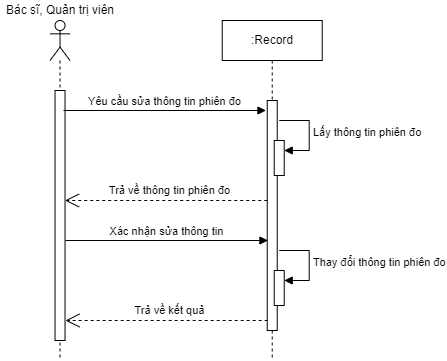
\includegraphics[width=10.5cm,height=9cm]{Images/sequence/sequence_manage_edit_record.png}
  \caption[Sơ đồ tuần tự chức năng sửa thông tin phiên đo]{\bfseries \fontsize{12pt}{0pt}
  \selectfont Sơ đồ tuần tự chức năng sửa thông tin phiên đo}
  \label{sequence_edit_record} %đặt tên cho ảnh
\end{figure}
Nếu bác sĩ, quản trị viên muốn sửa thông tin phiên đo, bác sĩ và quản trị viên gửi yêu cầu thay đổi, yêu cầu sẽ được xử lý bởi lớp Record, 
nếu có lỗi phát sinh sẽ trả về người dùng, nếu thay đổi thành công lớp Record sẽ gửi thông báo thành công. 

\begin{figure}[H]
  \centering
  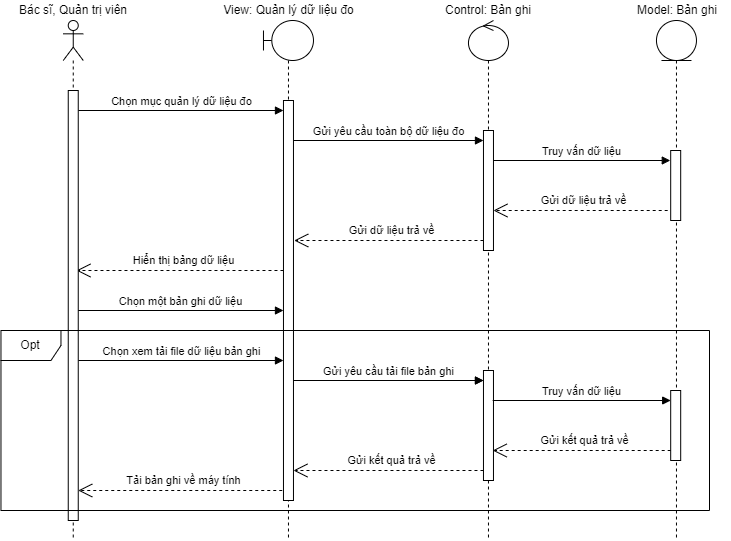
\includegraphics[width=10cm,height=9cm]{Images/sequence/sequence_download_records.png}
  \caption[Sơ đồ tuần tự chức năng tải bản ghi dữ liệu đo]{\bfseries \fontsize{12pt}{0pt}
  \selectfont Sơ đồ tuần tự chức năng tải bản ghi dữ liệu đo}
  \label{sequence_download_record} %đặt tên cho ảnh
\end{figure}
Nếu bác sĩ, quản trị viên muốn tải bản ghi dữ liệu đo, bác sĩ và quản trị viên gửi yêu cầu tải, yêu cầu sẽ được xử lý bởi lớp Record, 
nếu có lỗi phát sinh sẽ trả về người dùng, nếu thay đổi thành công lớp Record sẽ gửi file về máy tính. 
\subsubsection{Sơ đồ tuần tự chức năng quản lý dịch vụ nhắn tin}
\begin{figure}[H]
  \centering
  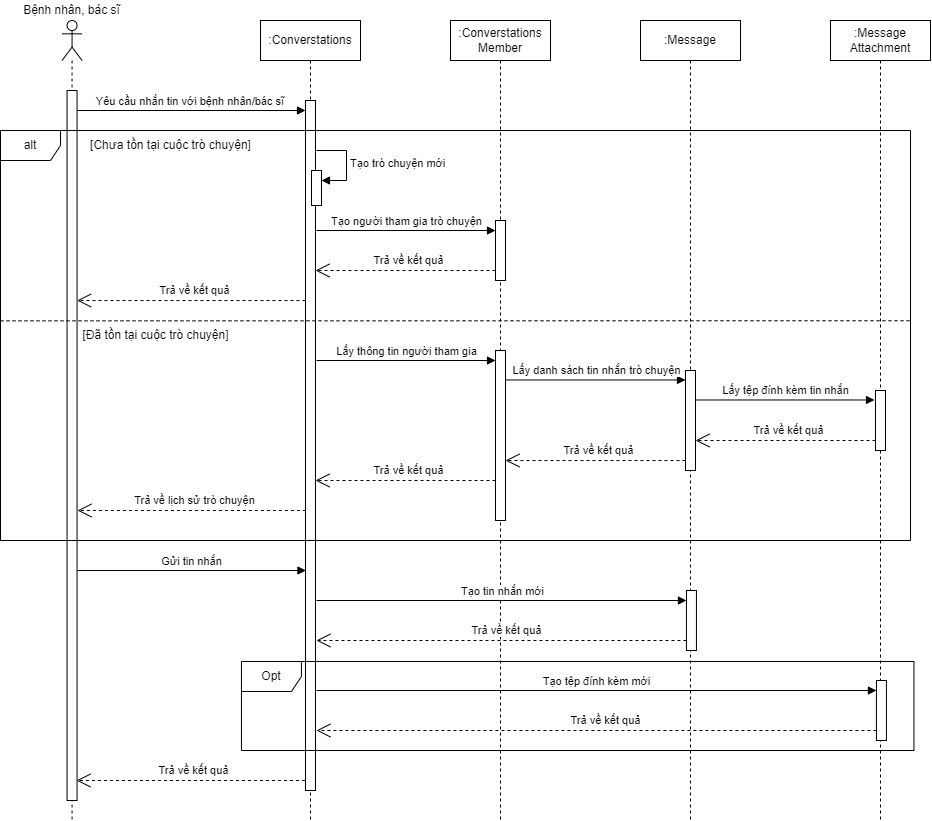
\includegraphics[width=15.5cm,height=14cm]{Images/sequence/sequence_chat.png}
  \caption[Sơ đồ tuần tự chức năng quản lý dịch vụ nhắn tin]{\bfseries \fontsize{12pt}{0pt}
  \selectfont Sơ đồ tuần tự chức năng quản lý dịch vụ nhắn tin}
  \label{sequence_chat} %đặt tên cho ảnh
\end{figure}
Sơ đồ tuần tự trên mô tả chi tiết quá trình người dùng xem và gửi tin nhắn giữa bệnh nhân và bác sĩ trên hệ thống. Người dùng gửi yêu cầu nhắn tin, 
chọn người mà mình muốn xem/gửi tin nhắn. Khi đó yêu cầu sẽ được xử lý bởi lớp Conversation, nếu người dùng đã có hội thoại sẽ trả về lịch sử đoạn hội thoại, ngược lại người dùng sẽ tạo cuộc hội thoại mới. 
Khi người dùng gửi tin nhắn, yêu cầu sẽ được xử lý bởi lớp Conversation gửi tin nhắn đến ngưởi nhận và lưu vào cơ sở dữ liệu.

\subsubsection{Sơ đồ tuần tự chức năng hỏi, nhận tư vấn từ trợ lý ảo}
\begin{figure}[H]
  \centering
  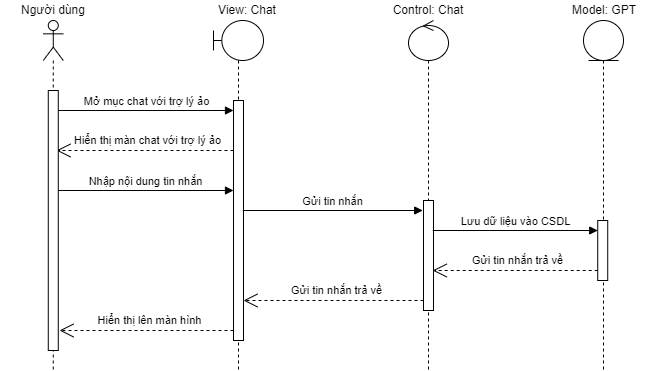
\includegraphics[width=15.5cm,height=11cm]{Images/sequence/sequence_chat_ai.png}
  \caption[Sơ đồ tuần tự chức năng hỏi, nhận tư vấn từ trợ lý ảo]{\bfseries \fontsize{12pt}{0pt}
  \selectfont Sơ đồ tuần tự chức năng hỏi, nhận tư vấn từ trợ lý ảo}
  \label{sequence_chat_ai} %đặt tên cho ảnh
\end{figure}
Sơ đồ tuần tự trên mô tả chi tiết quá trình người dùng xem và gửi tin nhắn với trợ lý ảo trên hệ thống. Người dùng chọn mở giao diện nhắn tin với trợ lý ảo, 
khi người dùng gửi tin nhắn đến trợ lý ảo, yêu cầu sẽ được xử lý bởi lớp Conversation gửi đến trợ lý ảo và phản hồi lại câu trả lời từ trợ lý ảo.

\subsubsection{Sơ đồ tuần tự chức năng quản lý thiết bị}
\begin{figure}[H]
  \centering
  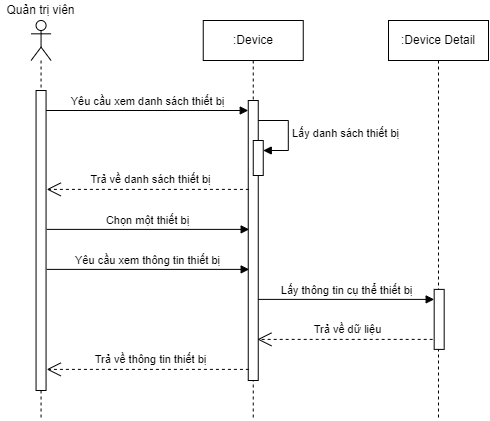
\includegraphics[width=11cm,height=9cm]{Images/sequence/sequence_manage_device.png}
  \caption[Sơ đồ tuần tự chức năng xem danh sách thiết bị]{\bfseries \fontsize{12pt}{0pt}
  \selectfont Sơ đồ tuần tự chức năng xem danh sách thiết bị}
  \label{sequence_manage_device} %đặt tên cho ảnh
\end{figure}
Sơ đồ tuần tự trên mô tả chi tiết quá trình quản trị viên xem danh sách thiết bị trên hệ thống. Quản trị viên gửi yêu cầu xem danh sách thiết bị, 
yêu cầu sẽ được xử lý bởi lớp Device, hiện danh sách thiết bị, quản trị viên có thể chọn một thiết bị và xem thông tin của họ. 
\begin{figure}[H]
  \centering
  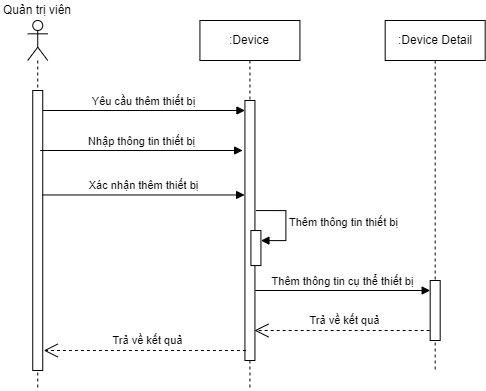
\includegraphics[width=11cm,height=8cm]{Images/sequence/sequence_manage_add_device.png}
  \caption[Sơ đồ tuần tự thêm thiết bị]{\bfseries \fontsize{12pt}{0pt}
  \selectfont Sơ đồ tuần tự thêm thiết bị}
  \label{sequence_manage_add_device} %đặt tên cho ảnh
\end{figure}
Nếu quản trị viên muốn tạo một thiết bị mới, quản trị viên nhập các thông tin và gửi yêu cầu tạo, yêu cầu sẽ được xử lý bởi lớp Device, nếu có lỗi phát sinh sẽ trả về quản trị viên, 
nếu tạo thành công lớp Device sẽ gửi kết quả trả về. 
\begin{figure}[H]
  \centering
  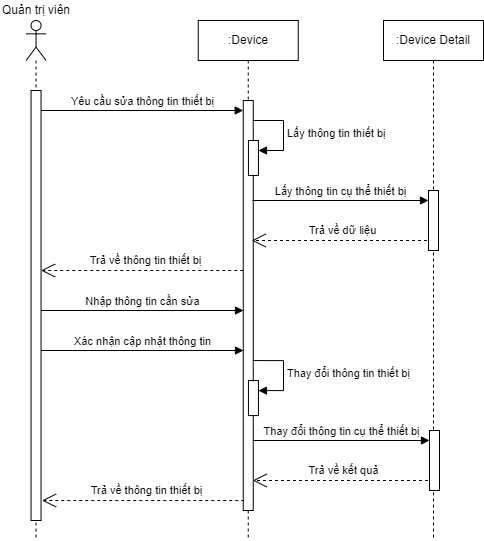
\includegraphics[width=11cm,height=12cm]{Images/sequence/sequence_manage_edit_device.png}
  \caption[Sơ đồ tuần tự chức năng sửa thông tin thiết bị]{\bfseries \fontsize{12pt}{0pt}
  \selectfont Sơ đồ tuần tự chức năng sửa thông tin thiết bị}
  \label{sequence_manage_edit_device} %đặt tên cho ảnh
\end{figure}
Nếu quản trị viên muốn chỉnh sửa thông tin thiết bị, quản trị viên nhập các thông tin cần sửa và gửi yêu cầu thay đổi, yêu cầu sẽ được xử lý
bởi lớp Device, nếu có lỗi phát sinh sẽ trả về quản trị viên, nếu thay đổi thành công Control sẽ gửi thông báo thành công. 
\begin{figure}[H]
  \centering
  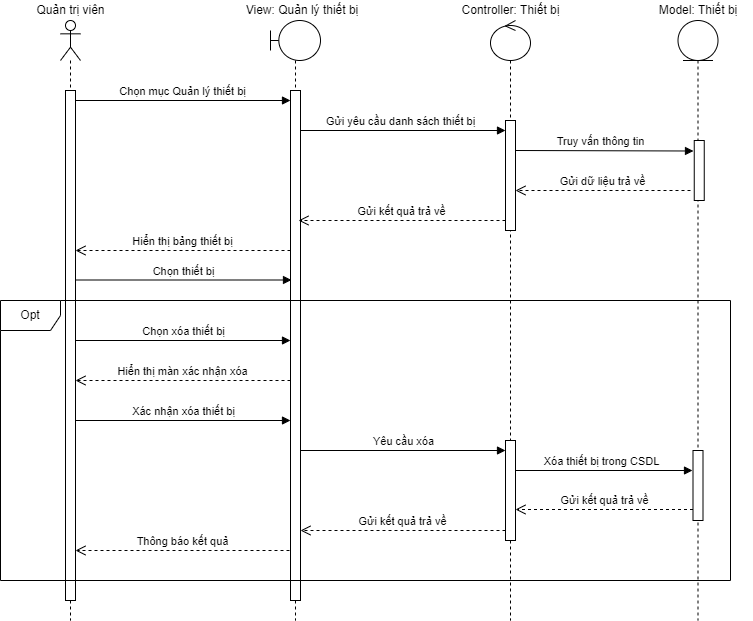
\includegraphics[width=11cm,height=8cm]{Images/sequence/sequence_manage_delete_device.png}
  \caption[Sơ đồ tuần tự chức năng xóa thiết bị]{\bfseries \fontsize{12pt}{0pt}
  \selectfont Sơ đồ tuần tự chức năng xóa thiết bị}
  \label{sequence_manage_delete_device} %đặt tên cho ảnh
\end{figure}
Nếu quản trị viên yêu cầu xóa thiết bị, lớp Device sẽ xử lý xóa thiết bị ở cơ sở dữ liệu và trả về thông báo cho quản trị viên.


\subsubsection{Sơ đồ tuần tự chức năng quản lý phân công bác sĩ - bệnh nhân}
\begin{figure}[H]
  \centering
  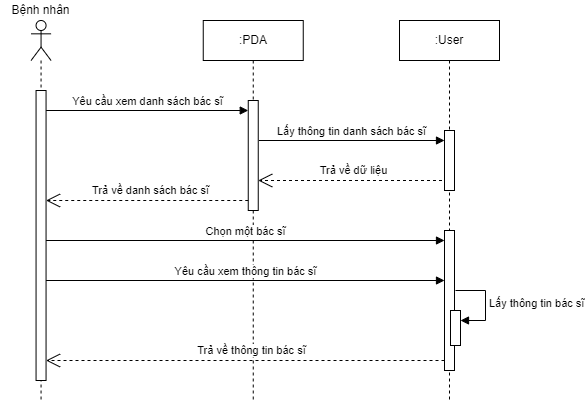
\includegraphics[width=13cm,height=9.5cm]{Images/sequence/sequence_manage_doctor.png}
  \caption[Sơ đồ tuần tự chức năng xem danh sách bác sĩ]{\bfseries \fontsize{12pt}{0pt}
  \selectfont Sơ đồ tuần tự chức năng xem danh sách bác sĩ}
  \label{sequence_manage_doctor} %đặt tên cho ảnh
\end{figure}
Sơ đồ tuần tự trên mô tả chi tiết quá trình bệnh nhân xem danh sách bác sĩ phụ trách mình trên hệ thống. Bệnh nhân gửi yêu cầu xem danh sách bác sĩ, 
yêu cầu sẽ được xử lý bởi lớp PDA, trả về danh sách bác sĩ, bệnh nhân có thể chọn một bác sĩ và xem thông tin của họ. 
\begin{figure}[H]
  \centering
  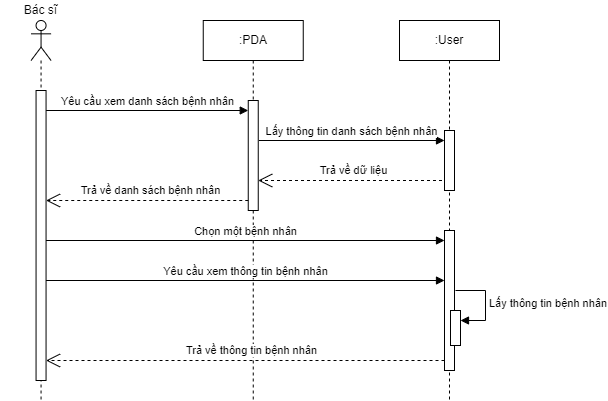
\includegraphics[width=12cm,height=8.5cm]{Images/sequence/sequence_manage_patient.png}
  \caption[Sơ đồ tuần tự chức năng xem danh sách bệnh nhân]{\bfseries \fontsize{12pt}{0pt}
  \selectfont Sơ đồ tuần tự chức năng xem danh sách bệnh nhân}
  \label{sequence_manage_patient} %đặt tên cho ảnh
\end{figure}
Sơ đồ tuần tự trên mô tả chi tiết quá trình bác sĩ xem danh sách bệnh nhân trên hệ thống. Bác sĩ gửi yêu cầu xem danh sách bệnh nhân, 
yêu cầu sẽ được xử lý bởi lớp PDA, trả về danh sách bệnh nhân, bác sĩ có thể chọn một bệnh nhân và xem thông tin của họ. 

\begin{figure}[H]
  \centering
  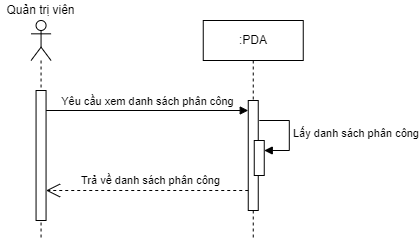
\includegraphics[width=9cm,height=6cm]{Images/sequence/sequence_manage_pda.png}
  \caption[Sơ đồ tuần tự chức năng xem danh sách phân công bác sĩ - bệnh nhân]{\bfseries \fontsize{12pt}{0pt}
  \selectfont Sơ đồ tuần tự chức năng xem danh sách phân công bác sĩ - bệnh nhân}
  \label{sequence_manage_pda} %đặt tên cho ảnh
\end{figure}
Sơ đồ tuần tự trên mô tả chi tiết quá trình quản trị viên xem danh sách phân công bác sĩ - bệnh nhân trên hệ thống. Quản trị viên gửi yêu cầu
xem danh sách phân công bác sĩ - bệnh nhân, yêu cầu sẽ được xử lý bởi lớp PDA, trả về danh sách phân công bác sĩ - bệnh nhân. 

\begin{figure}[H]
  \centering
  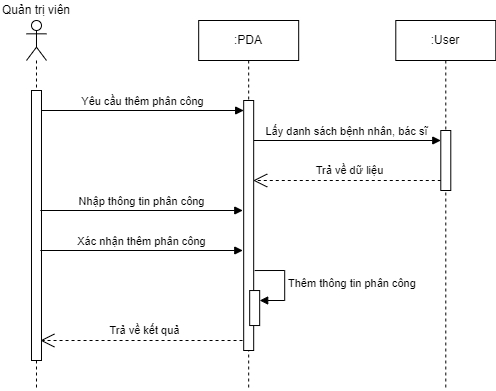
\includegraphics[width=11cm,height=8cm]{Images/sequence/sequence_manage_add_pda.png}
  \caption[Sơ đồ tuần tự chức năng thêm phân công bác sĩ - bệnh nhân]{\bfseries \fontsize{12pt}{0pt}
  \selectfont Sơ đồ tuần tự chức năng thêm phân công bác sĩ - bệnh nhân}
  \label{sequence_manage_add_pda} %đặt tên cho ảnh
\end{figure}
Sơ đồ tuần tự trên mô tả chi tiết quá trình quản trị viên tạo với danh sách phân công bác sĩ - bệnh nhân trên hệ thống. Quản trị viên gửi yêu cầu
thêm phân công bác sĩ - bệnh nhân, yêu cầu sẽ được xử lý bởi lớp PDA, nếu có lỗi phát sinh sẽ trả về người dùng, nếu thêm thành công sẽ gửi thông báo thành công.

\begin{figure}[H]
  \centering
  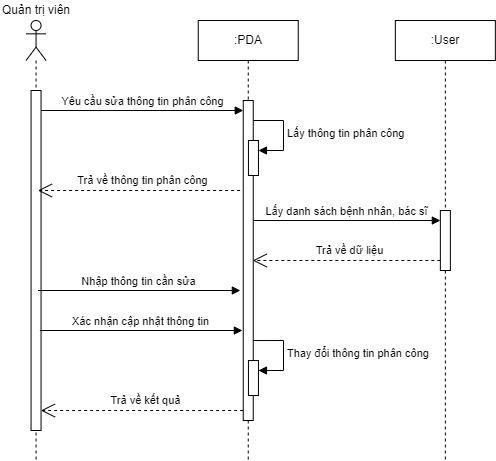
\includegraphics[width=11cm,height=10cm]{Images/sequence/sequence_manage_edit_pda.png}
  \caption[Sơ đồ tuần tự chức năng sửa thông tin phân công bác sĩ - bệnh nhân]{\bfseries \fontsize{12pt}{0pt}
  \selectfont Sơ đồ tuần tự chức năng sửa thông tin phân công bác sĩ - bệnh nhân}
  \label{sequence_manage_edit_pda} %đặt tên cho ảnh
\end{figure}
Nếu quản trị viên muốn chỉnh sửa thông tin phân công bác sĩ - bệnh nhân, quản trị viên gửi yêu cầu thay đổi, 
yêu cầu sẽ được xử lý bởi lớp PDA, nếu có lỗi phát sinh sẽ trả về người dùng, nếu thành công sẽ gửi thông báo thành công. 
\begin{figure}[H]
  \centering
  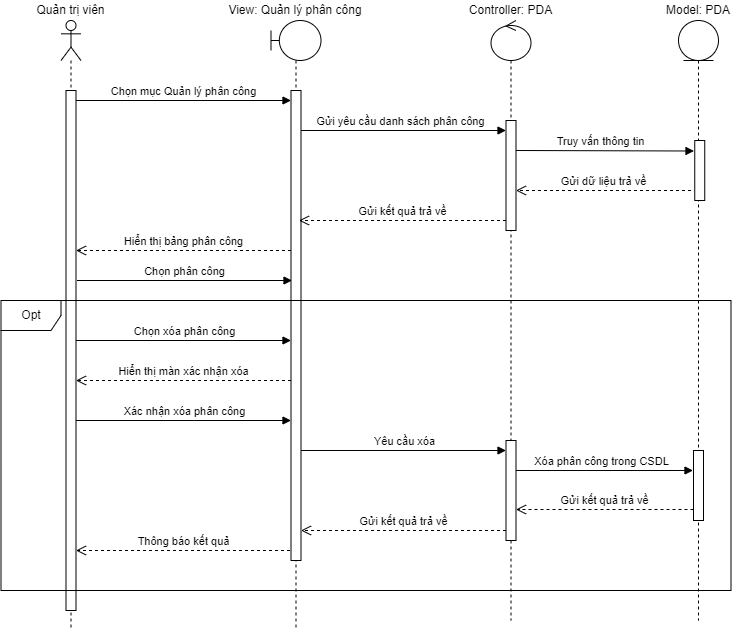
\includegraphics[width=9cm,height=7cm]{Images/sequence/sequence_manage_delete_pda.png}
  \caption[Sơ đồ tuần tự chức năng xóa phân công bác sĩ - bệnh nhân]{\bfseries \fontsize{12pt}{0pt}
  \selectfont Sơ đồ tuần tự chức năng xóa phân công bác sĩ - bệnh nhân}
  \label{sequence_manage_delete_pda} %đặt tên cho ảnh
\end{figure}
Nếu quản trị viên yêu cầu xóa phân công bác sĩ - bệnh nhân, lớp PDA sẽ xử lý xóa phân công ở cơ sở dữ liệu và trả về thông báo cho quản trị viên.

\subsubsection{Sơ đồ tuần tự chức năng quản lý tài khoản người dùng}
\begin{figure}[H]
  \centering
  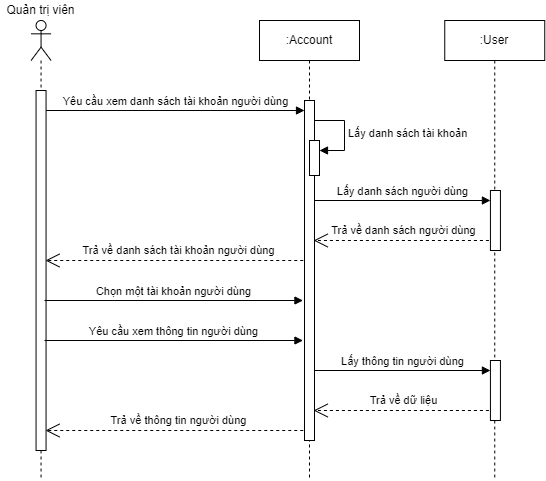
\includegraphics[width=11.5cm,height=10cm]{Images/sequence/sequence_manage_user.png}
  \caption[Sơ đồ tuần tự chức năng xem danh sách tài khoản người dùng]{\bfseries \fontsize{12pt}{0pt}
  \selectfont Sơ đồ tuần tự chức năng xem danh sách tài khoản người dùng}
  \label{sequence_manage_user} %đặt tên cho ảnh
\end{figure}
Sơ đồ tuần tự trên mô tả chi tiết quá trình quản trị viên xem danh sách tài khoản người dùng trên hệ thống. Quản trị viên yêu cầu xem
quản lý tài khoản người dùng, yêu cầu sẽ được xử lý bởi lớp User, trả về danh sách tài khoản người dùng, quản trị viên có thể chọn một người dùng và xem thông tin của họ. 
\begin{figure}[H]
  \centering
  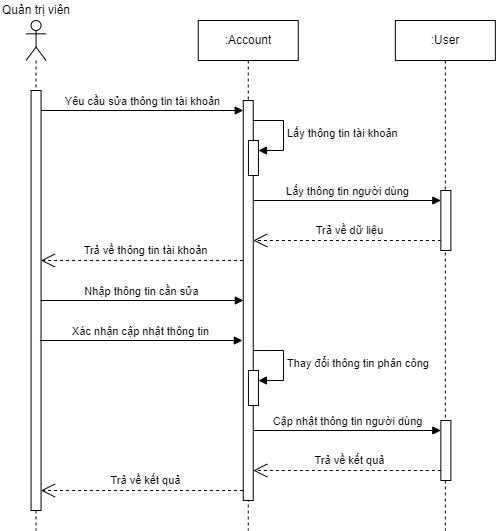
\includegraphics[width=12cm,height=12cm]{Images/sequence/sequence_manage_edit_user.png}
  \caption[Sơ đồ tuần tự chức năng sửa thông tin người dùng]{\bfseries \fontsize{12pt}{0pt}
  \selectfont Sơ đồ tuần tự chức năng sửa thông tin người dùng}
  \label{sequence_manage_edit_user} %đặt tên cho ảnh
\end{figure}
Nếu quản trị viên muốn chỉnh sửa thông tin người dùng, quản trị viên gửi yêu cầu thay đổi, yêu cầu sẽ được xử lý bởi lớp User, nếu có lỗi phát sinh sẽ hiển thị lên màn hình,
nếu thay đổi thành công lớp User sẽ gửi thông báo thành công. 
\begin{figure}[H]
  \centering
  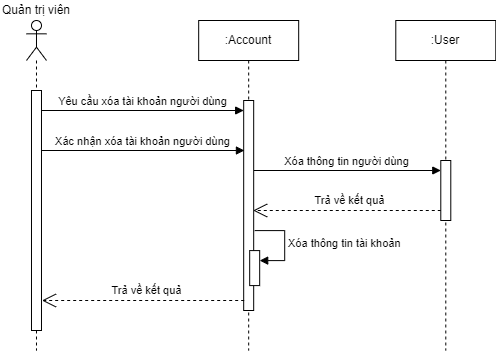
\includegraphics[width=10cm,height=7.5cm]{Images/sequence/sequence_manage_delete_user.png}
  \caption[Sơ đồ tuần tự chức năng xóa người dùng]{\bfseries \fontsize{12pt}{0pt}
  \selectfont Sơ đồ tuần tự chức năng xóa người dùng}
  \label{sequence_manage_delete_user} %đặt tên cho ảnh
\end{figure}
Nếu quản trị viên yêu cầu xóa tài khoản người dùng, lớp User sẽ xử lý xóa tài khoản ở cơ sở dữ liệu và trả về thông báo cho quản trị viên.
\begin{figure}[H]
  \centering
  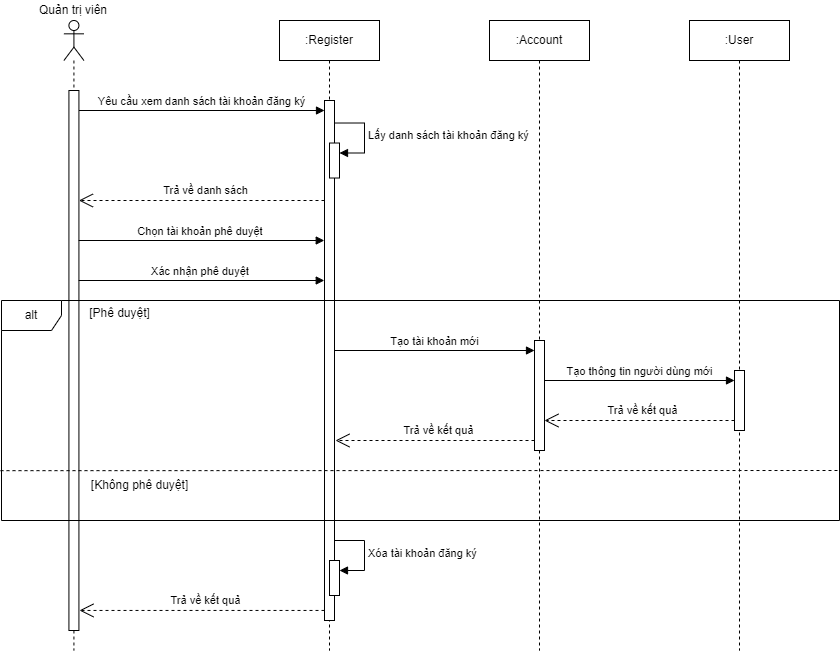
\includegraphics[width=14.5cm,height=13cm]{Images/sequence/sequence_manage_register.png}
  \caption[Sơ đồ tuần tự chức năng phê duyệt tài khoản người dùng]{\bfseries \fontsize{12pt}{0pt}
  \selectfont Sơ đồ tuần tự chức năng phê duyệt tài khoản người dùng}
  \label{sequence_manage_register} %đặt tên cho ảnh
\end{figure}
Nếu quản trị viên muốn phê duyệt tài khoản người dùng, quản trị sẽ chọn phê duyệt hoặc không phê duyệt, yêu cầu sẽ được xử lý bởi lớp Register, nếu có lỗi phát sinh sẽ trả về quản trị viên,
nếu phê duyệt thành công lớp Register sẽ gửi thông báo thành công. 

\subsection{Phân tích dữ liệu}

Tại phần này, chúng em sẽ tiến hành xác định và mô tả các thực thể cũng như
 thuộc tính trong hệ thống. Việc này giúp chúng em có thể nắm được các phần chính 
 trong việc thiết kế nên cơ sở dữ liệu.

     Đầu tiên, chúng em sẽ xác định các thực thể và mô tả thuộc tính của nó trong hệ
      thống dươi dạng bảng và sơ đồ mô hình liên kết. 

\begin{table}[H]
  \caption{\bfseries \fontsize{12pt}{0pt}\selectfont Bảng thực thể và thuộc tính}
  \centering
  \begin{tabularx}{0.9\textwidth}{|c|X|}
    \hline
    \textbf{Thực thể} & \textbf{Thuộc tính} \\
    \hline
    Người dùng & 
    ID người dùng, Tên người dùng, Ngày sinh, Giới tính, Số điện thoại, Quyền, Trạng thái, Đường dẫn lưu trữ ảnh, Thông tin người dùng \\
    \hline
    Tài khoản &
    ID tài khoản, Email, Mật khẩu  \\
    \hline
    Token đăng nhập &
    ID token, Token truy cập, Token làm mới \\
    \hline
    Thiết bị & 
    ID thiết bị, Tên thiết bị, Loại thiết bị, Thông tin thiết bị, Trạng thái thiết bị, Ngày bắt đầu sử dụng\\
    \hline
    Thông số thiết bị &
    ID thông số, Tên thông số, Giá trị thông số, Thông tin cụ thể, Loại thông số \\
    \hline
    Bản ghi dữ liệu & 
    ID bản ghi dữ liệu, Loại bản ghi, Đường dẫn lưu trữ dữ liệu, Thời gian bắt đầu đo, Thời gian kết thúc đo \\
    \hline
    Thông tin hội thoại &
    ID hội thoại, Tên hội thoại, Loại hội thoại, Đường dẫn avatar hội thoại \\
    \hline
    Thành viên tham gia hội thoại &
    ID thành viên tham gia, Trạng thái thông báo (Có thông báo, Không thông báo), Tác vụ (người tạo đoạn hội thoại, thành viên trong đoạn hội thoại), Trạng thái đã xem\\
    \hline
    Tin nhắn & 
    ID tin nhắn, Nội dung tin nhắn, Tin nhắn hệ thống, Ghim (tin nhắn được ghim, không được ghim), Thời gian ghim tin nhắn, Các lượt thả cảm xúc \\
    \hline
    Tệp đính kèm &
    ID tệp đính kèm, Đường dẫn tệp, Tên tệp, Kích thước tệp, Đường dẫn thumbnail, Loại đính kèm (hình ảnh, video, tệp tin) \\
    \hline 
    Phân công bệnh nhân - bác sĩ & 
    ID phân công, ID bệnh nhân, ID bác sĩ, Ngày bắt đầu, Ngày kết thúc \\
    Tài khoản phê duyệt & 
    ID tài khoản phê duyệt, Email, Mật khẩu, Tên người dùng, Ngày sinh, Giới tính, Số điện thoại, Quyền, Trạng thái, Đường dẫn lưu trữ ảnh, Thông tin người dùng \\
    \hline
  \end{tabularx}

  
\end{table}
Sau khi hoàn thành được bảng thực thể và thuộc tính, chúng em xác định được mô hình thực thể liên kết như sau:

\begin{figure}[H]
  \centering
  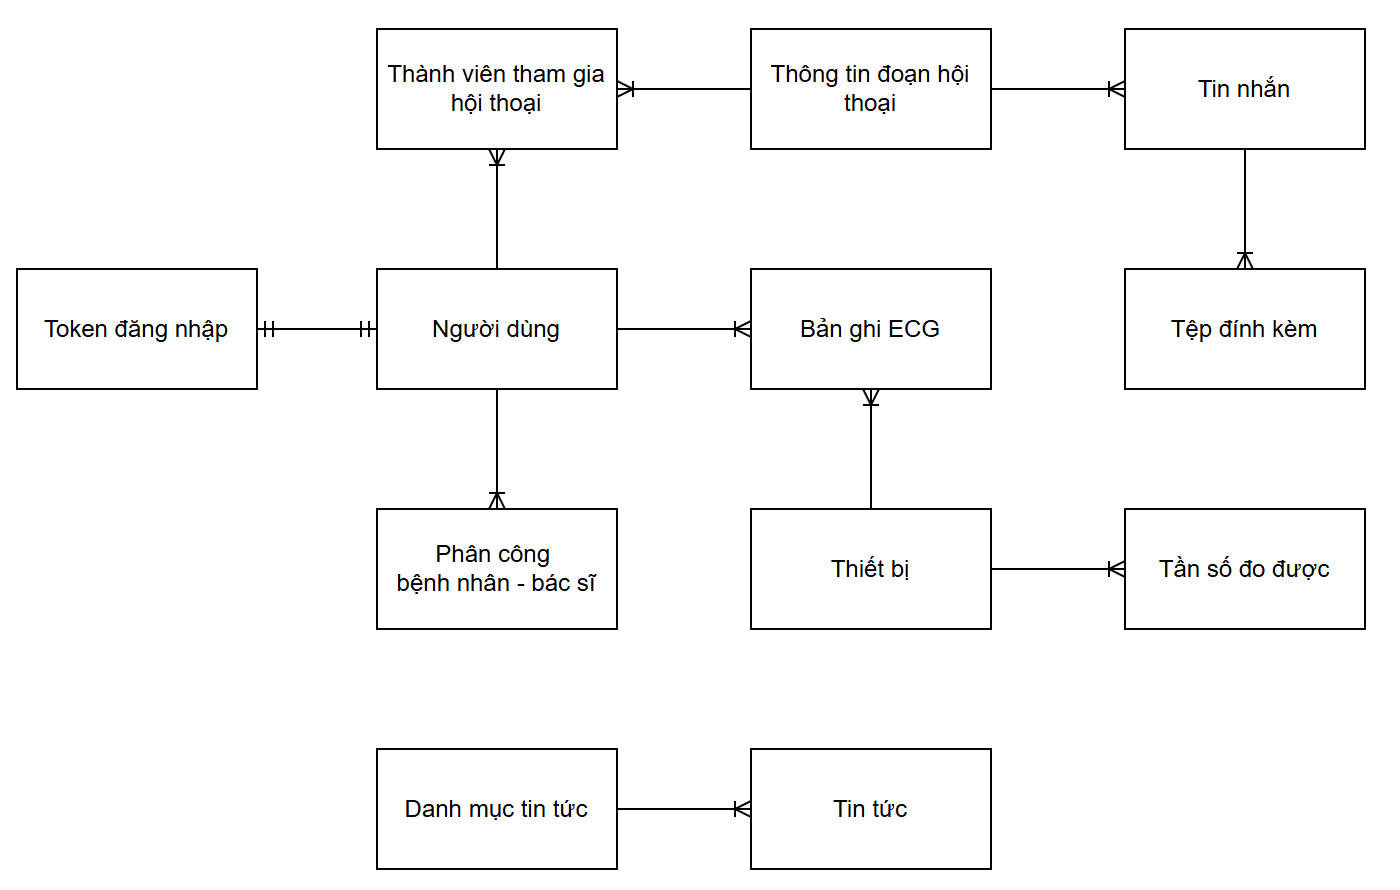
\includegraphics[width=15cm,height=9.5cm]{Images/system/fmECG_connection_entity.png}
  \caption[Mô hình thực thể liên kết]{\bfseries \fontsize{12pt}{0pt}
  \selectfont Mô hình thực thể liên kết}
  \label{ttlk} %đặt tên cho ảnh
\end{figure}

\subsection{Kết luận}

Chương này thực hiện phân tích khái quát về
 hệ thống, nhằm đáp ứng các yêu cầu và mục tiêu đã được đề ra trong các phần trên.

\newpage
